\section{Introduction to Neutrinos}
In 1914, James Chadwick measured the energy spectrum of outgoing electrons in beta decay and showed that the spectrum was continuous~\cite{ChadwickSource}, though it was expected to consist of one discrete, well defined value due to the presumed two-body nature of the decay. While some chose to believe that a lack of energy conservation is the underlying cause of the continuous spectrum, in 1930 Pauli proposed (translated from German) ~\cite{PauliLetter}:
\begin{displayquote}
``...in the nuclei there could exist electrically neutral particles, which I will call neutrons, that have spin 1/2 and obey the exclusion principal and that further differ from light quanta in that they do not travel with the velocity of light... The continuous beta spectrum would then make sense with the assumption that in beta decay, in addition to the electron, a neutron is emitted such that the sum of the energies of neutron and electron is constant.''
\end{displayquote}
Though Pauli named the particle a ``neutron'' (a name later used for the subatomic particle comprised of two down quarks and one up quark), his prediction was otherwise correct. Only 26 years later in 1956, the first neutrino was observed.\\

Neutrinos make up three of the six leptons in the Standard Model of particle physics. There are three flavor eigenstates, each of which are paired to one of the other three leptons: electron neutrinos ($\nu_e$), muon neutrinos ($\nu_\mu$), and tau neutrinos ($\nu_\tau$). Each neutrino has an antiparticle partner, the antineutrino. Neutrinos are particularly elusive because they are electrically neutral and only interact through the weak interaction and gravity. The number of active neutrino flavors is constrained to three (2.984 $\pm$ 0.0082) by precision measurements of the $Z$ decay width~\cite{ZDecayWidthsource}. \\

The flavor of a neutrino is determined by measuring the outgoing lepton in charged current neutrino interactions. In such an interaction, a $\nu_e$ produces an electron, a $\nu_\mu$ produces a muon, and a $\nu_\tau$ produces a tau.\\

\section{Neutrino Oscillations}
It was until 1968 that neutrinos were widely believed to be massless. In this year, Ray Davis and collaborators were measuring neutrinos originating from within the sun (``solar neutrinos'') by studying charged-current $\nu_e$ interactions on chlorine atoms. They measured only one third as many neutrino interactions as expected, a fact which wasn't fully understood until 2001. By combining results from other experiments (including from the Kamiokande experiment in Japan measuring a deficit of $\nu_\mu$ from cosmic ray interactions in the atmosphere in 1998~\cite{KamiokandeOscsource}, and from the Sudbury Neutrino Observatory (SNO) experiment ~\cite{SNOOscsource}), the idea that neutrinos oscillated from one flavor to another became widely accepted.\\

Neutrino oscillations occur when a neutrino produced as one flavor eigenstate changes to another flavor eigenstate after propagating a distance, $L$. Oscillation is only possible because the three mass eigenstates are non-zero and are different than the three flavor eigenstates. Neutrino propagation happens as a mixture of mass eigenstates with different DeBroglie wavelengths, which constructively and destructively interfere with one another. The mass eigenstates are referred to as $\nu_1$, $\nu_2$, and $\nu_3$ with masses $m_1$, $m_2$, and $m_3$ respectively. While the absolute masses are yet unknown, the mass-squared splitting between the masses have been measured ($\Delta m_{i,j} = m_j^2-m_i^2$). This introduces two possible ordering configurations of the neutrino masses: the ``normal'' hierarchy in which $m_1<m_2<m_3$, and the ``inverted'' hierarchy, in which $m_3<m_1<m_2$. The two hierarchy possibilities are depicted in Figure \ref{nu_hierarchy_fig}~\cite{HierarchyFigsource}. As seen in the figure, the larger of the two mass splittings is referred to as $\Delta m^2_{\text{atm}}$ and the smaller of the two is referred to $\Delta m^2_{\text{sol}}$ because they are generally measured with atmospheric neutrinos or solar neutrinos, respectively.\\

\begin{figure}[ht!]
\centering
	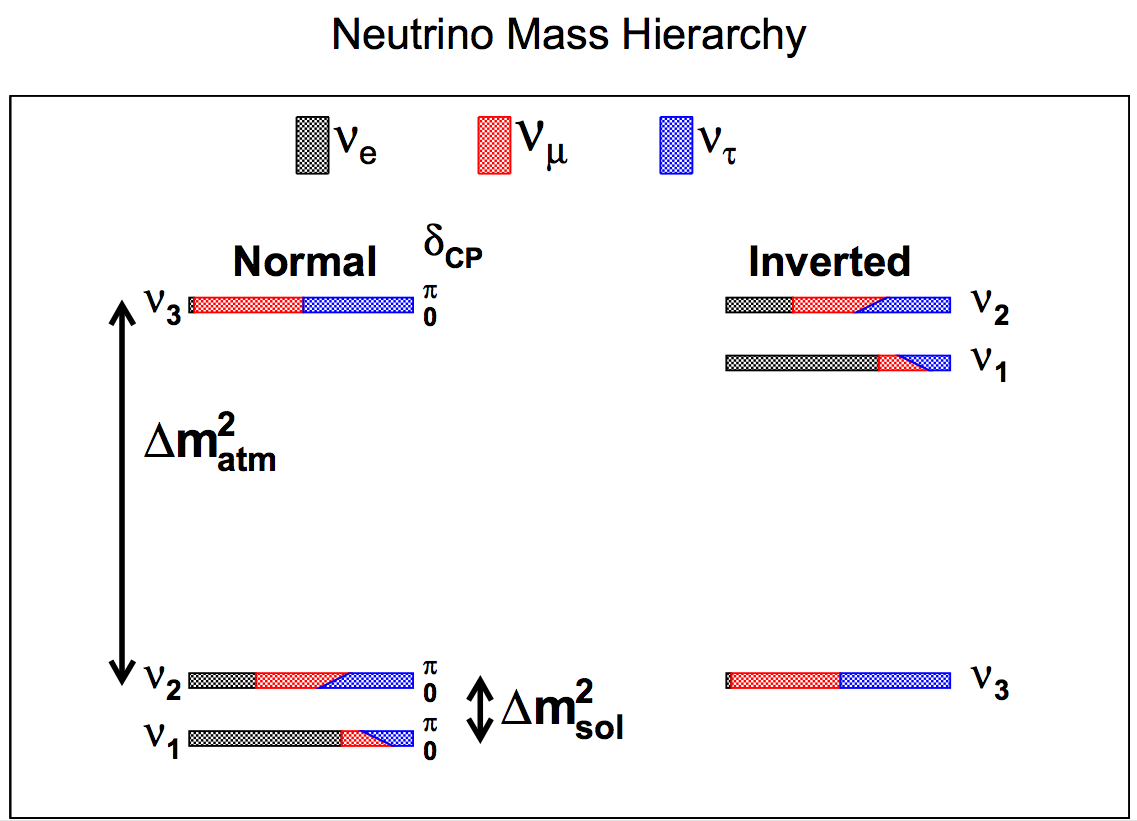
\includegraphics[width=0.9\textwidth]{Figures/nu_hierarchy_fig.png} \\
\caption{\textit{The neutrino mass hierarchy possibilities. The flavor eigenstate fraction for each mass eigenstate is shown by the relative amount of gray, red, or blue in each bar.}}\label{nu_hierarchy_fig}
\end{figure}

A neutrino mass eigenstate can be expressed as a quantum superposition of flavor eigenstates by way of the Pontecorvo-Maki-Nakagawa-Sakata (PMNS) $3\times3$ unitary mixing matrix, $U$:
\begin{equation}\label{nuPMNSmixeqtn}
\Ket{\nu_i} = \sum_\alpha^3 U_{i,\alpha}\Ket{\nu_\alpha}
\end{equation}
where $\Ket{\nu_i}$ represents the $i$th mass eigenstate ($i=1,2,3$) and $\Ket{\nu_\alpha}$ represents the flavor eigenstate ($\alpha=e,\mu,\tau$). Generally the PMNS matrix is factorized into three matrices parameterized by four parameters: three mixing angles $\theta_{12}$, $\theta_{23}$, $\theta_{13}$, and one CP violating phase $\delta$.

\begin{equation}\label{PMNSfactorized}
U = \begin{bmatrix} 1 & 0 & 0 \\ 0 & c(\theta_{23}) & s(\theta_{23}) \\ 0 & -s(\theta_{23}) & c(\theta_{23}) \end{bmatrix} 
\begin{bmatrix} c(\theta_{13}) & 0 & s(\theta_{13})e^{-i\delta} \\ 0 & 1 & 0 \\ -s(\theta_{13})e^{-i\delta} & 0 & c(\theta_{13}) \end{bmatrix} 
\begin{bmatrix} c(\theta_{12}) & s(\theta_{12}) & 0 \\ -s(\theta_{12}) & c(\theta_{12}) & 0 \\ 0 & 0 & 1 \end{bmatrix} 
\end{equation}

where ``c'' stands for $\cos$ and ``s'' stands for $\sin$.\\

In general, an experiment searching for neutrino oscillations has the choice of searching for appearance or disappearance. In appearance experiments, a neutrino of one known flavor is produced (flavor $\alpha$), and one attempts to measure that neutrino as another flavor (flavor $\beta$). Appearance searches have the added benefit of potentially shedding light on CP violation, which leads to appearance probabilities $P(\nu_\alpha\rightarrow\nu_\beta) \ne P(\overline{\nu}_\alpha\rightarrow\overline{\nu}_\beta)$. In a disappearance search, neutrinos of known flavor are produced at a known rate, and a decreased rate (deficit) of that same neutrino flavor is measured a distance away. Since $P(\nu_\alpha\rightarrow\nu_\alpha) = P(\overline{\nu}_\alpha\rightarrow\overline{\nu}_\alpha)$, disappearance searches allow for the combination of neutrino and anti-neutrino data for increased oscillation sensitivity.\\

A classic graduate-student quantum mechanical qualification exam question is to determine an oscillation probability assuming only two neutrinos. This can be parameterized with one effective mixing angle, $\theta$, and the nominal rotation matrix
\begin{equation}\label{rotmatrix}
U = \begin{bmatrix} \cos\theta & \sin\theta \\ -sin\theta & cos\theta \end{bmatrix}.
\end{equation}
A neutrino of flavor $\nu_\alpha$ will propagate as the superposition of the two mass eigenstates, $\nu_1$ and $\nu_2$
\begin{equation}\label{twonupropagation}
\Ket{\nu_\alpha (t)} = \cos(\theta)e^{-iE_1t}\ket{\nu_1} + \sin(\theta)e^{-iE_2t}\ket{\nu_2} 
\end{equation}
Using the relativistic approximation (which is valid for neutrinos of almost any momenta, $p$, given their small mass, $m$)
\begin{equation}\label{relapprox}
E_i = p_i + \frac{m_i^2}{2p_i}
\end{equation}
the oscillation probability for a neutrino of flavor $\alpha$ to be detected as flavor $\beta$ after traveling a distance L at approximately the speed of light is given by
\begin{equation}\label{twoneutrinooscprob0}
P_{\alpha \rightarrow \beta} = \left|\Bra{\nu_\alpha}\Ket{\nu_\beta}\right|^2 = \sin^2 2\theta \sin^2 \left( 1.27 \frac{\Delta m^2 L}{E} \right)
\end{equation}
where the $1.27$ factor comes from a proper handling of units including $\hbar$ and $c$. The $L/E$ frequency modulation of oscillations is characteristic of two neutrino measurements, for example as beautifully demonstrated by the KamLAND collaboration measuring $\Delta m_{21}^2$ and $\theta_{12}$ with nuclear reactor anti-neutrinos, as shown in Figure \ref{KAMLANDfig}~\cite{KAMLANDsource}.

\begin{figure}[ht!]
\centering
	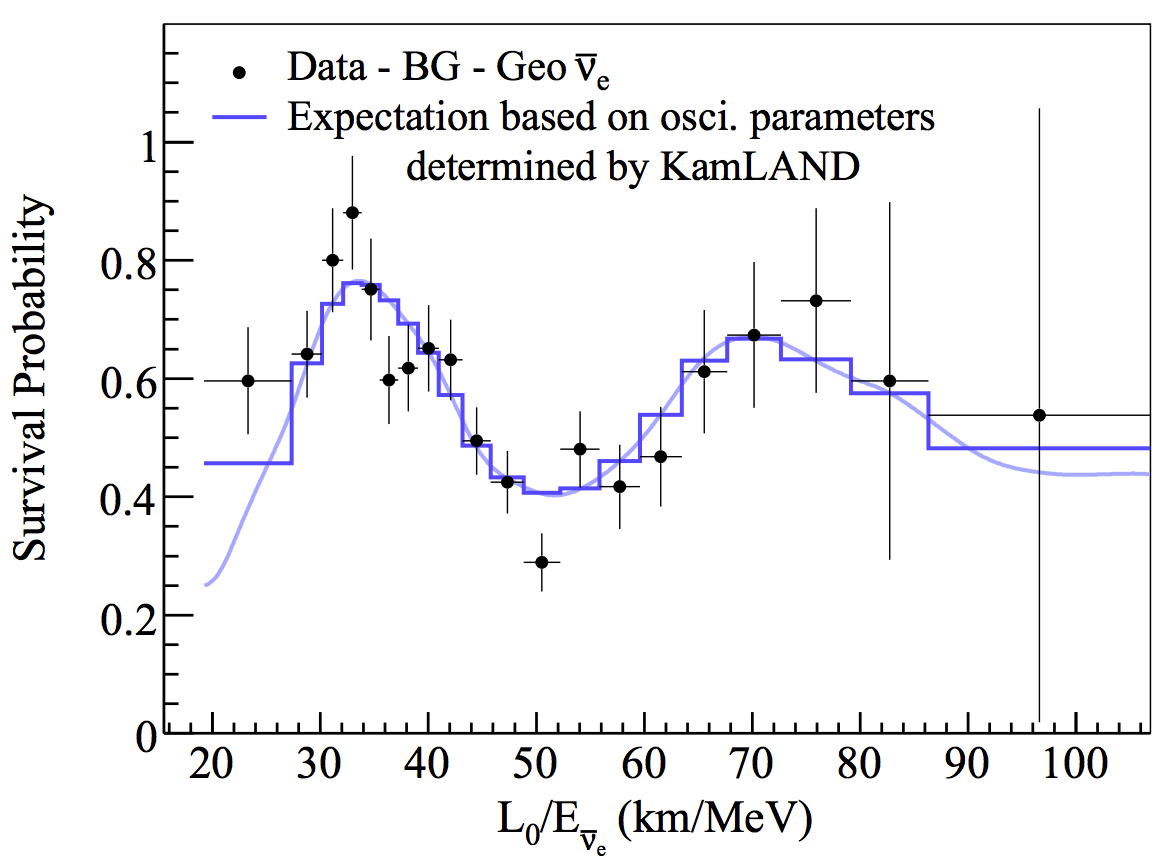
\includegraphics[width=0.9\textwidth]{Figures/KAMLANDfig.png} \\
\caption{\textit{Results from the KamLAND collaboration measuring the survival probability of $\overline{\nu}_e$ from nuclear reactors. A clear oscillation as a function of $L/E$ as predicted by the two-neutrino model is shown.}}\label{KAMLANDfig}
\end{figure}
% (Ref \protect\cite{KAMLANDsource}})

\section{Sterile Neutrinos}
While is is well known that there are only three active neutrino flavor states from the measured width of the $Z$ decay, it is possible to introduce one or more ``sterile'' neutrino states which do not couple weakly. Each addition of a sterile neutrino adds a row and column to the PMNS mixing matrix, and a new sterile mass eigenstate is defined as
\begin{equation}\label{sterilenuPMNSmixeqtn}
\Ket{\nu_s} = \sum_\alpha^{3+N} U_{i,\alpha}\Ket{\nu_\alpha}
\end{equation}
where $N$ is the number of additional sterile neutrinos added to the model.\\

Proposing the existence of one or more sterile neutrino eigenstates was inspired by the results of the LSND and MiniBooNE experiments, which are discussed in more detail in Chapter \ref{sec:LEEhistory}. LSND observed an excess of $\overline{\nu}_e$-like interactions in a $\overline{\nu}_\mu$ beam~\cite{LSNDPaper}. When fit to the three-neutrino oscillation model, the excess strongly disagreed with other measurements of neutrino mixing angles and $\Delta m^2$ values. The fit value of $\Delta m^2$ was on the order of 1 $eV^2$, orders of magnitude higher than previously measured values of $\Delta m_{12}^2$ and $\Delta m_{23}^2$. The existence of one or more sterile neutrinos could explain this drastically different measured $\Delta m^2$ value, since new additional mass eigenstate(s) are included in the propagating superposition, therefore changing neutrino oscillation probabilities. Including this measured sterile neutrino mass splitting in the ``normal'' or ``inverted'' hierarchy is shown in Figure \ref{sterile_nu_hierarchy_fig}~\cite{GaryThesis}.\\

\begin{figure}[ht!]
\centering
	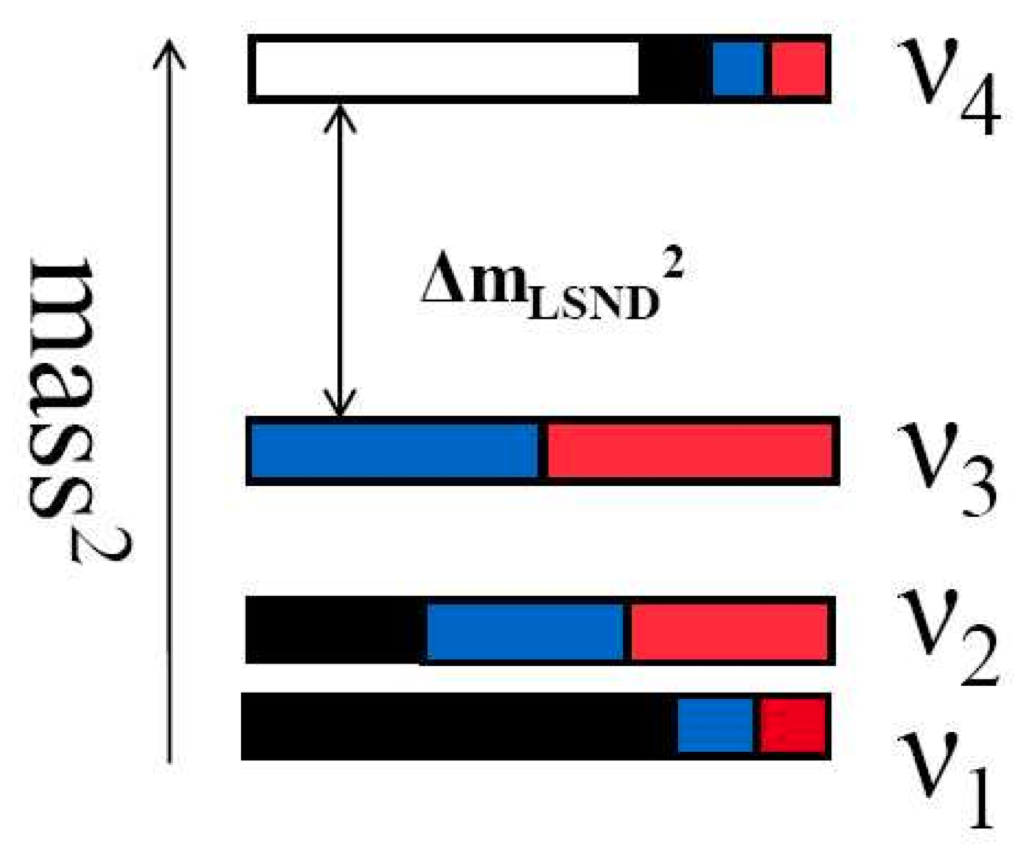
\includegraphics[width=0.7\textwidth]{Figures/sterile_masssplitting.png} \\
\caption{\textit{Mass hierarchy with one heavy sterile neutrino included. The $\delta m^2$ from LSND is incorporated.}}\label{sterile_nu_hierarchy_fig}
\end{figure}

Following the LSND experiment, the MiniBooNE experiment was proposed to search for oscillations with a similar mass splitting to that measured by LSND. In 2010, MiniBooNE observed a two anti-neutrino oscillation appearance-only measurement consistent with LSND over the null oscillation hypothesis at the 98\% confidence level.\\

The following chapter of this thesis provides an introduction to the MicroBooNE detector, which was proposed to search for the same MiniBooNE excess but with a different detector technology.
